\label{sec:local}

Pour un état initial du gaz correspondant à un facteur d'occupation lisse $\nu(\theta)$ (par exemple un état thermique), le facteur d'occupation $\nu^*(x/t,\theta)$ à rapport $x/t$ fixé est attendu comme étant fortement asymétrique en fonction de $\theta$, selon l'équation~\eqref{eq:nuetoile}. En effet, du côté droite, il présente une discontinuité du type saut, similaire à celle du facteur d'occupation de l’état fondamental, tandis que du côté gauche, il reste lisse. Afin de révéler ces caractéristiques particulières de l’état local du gaz, nous utilisons le protocole introduit dans la Réf.~\cite{dubois_probing_2024} pour sonder la distribution locale des rapidités, comme expliqué ci-après.

Nous laissons d’abord le gaz se dilater pendant un temps $t=18~\mathrm{ms}$, de sorte que le bord s’étale sur une large zone d’environ $350~\mathrm{\mu m}$, comme illustré en Fig.~\ref{fig:BiPart.coupure1} (e)-(f) et  Fig ~\ref{fig:simul_deformation} (a).  
Nous sélectionnons ensuite une tranche du gaz comprise dans l’intervalle $[x_0-\ell/2, x_0+\ell/2]$, en éliminant tous les atomes situés hors de cette tranche à l’aide d’un faisceau de poussée~\cite{dubois_probing_2024}(Fig \ref{fig:BiPart.coupure2} (a)--(c)). 

\begin{figure}[!htb]
	\centering
	\includegraphics[width=\textwidth , page = 6 ]{Shema.pdf}
	\caption{
(a) À l'instant $\tau = 0^+$, immédiatement après la sélection de la tranche centrée en $x = x_0$ et de largeur $\ell$, la distribution de rapidité localement résolue est donnée par $\rho(x,\theta ; \tau = 0^+) = \nu(x, \theta ; t = 18~\mathrm{ms}) \, \rho_s(x,\theta ; t = 18~\mathrm{ms})$ pour $\vert x - x_0 \vert < \ell/2$, et est nulle pour $\vert x - x_0 \vert > \ell/2$. Le bord gauche immédiatement après la sélection est représenté en pointillés par l’ensemble des points $(x_g(s; \tau = 0^+),\ \theta_g(s; \tau = 0^+))$, et le bord droit en tiret-point par l’ensemble des points $(x_d(s; \tau = 0^+),\ \theta_d(s; \tau = 0^+))$. Le bord complet est donc la concaténation de ces deux ensembles. 
(b) Densité linéique spatiale $\tilde{n}(x)$ : en pointillés, $n(x; t = 18~\mathrm{ms})$ juste avant la sélection ; en ligne pleine, $\tilde{n}(x; \tau = 0^+)$, égal à $n(x; t = 18~\mathrm{ms})$ pour $\vert x - x_0 \vert < \ell/2$ et nul ailleurs. 
(c) Distribution de rapidité après sélection, $\Pi(\theta) = \int \rho(x,\theta ; \tau)\,\mathrm{d}x$, invariante sous l’évolution unidimensionnelle, représentée en rouge. La distribution localement résolue en $x_b(s; \tau = 0^+)$, $\rho(x_b(s; \tau = 0^+), \theta ; \tau = 0^+)$, est représentée en pointillés. Cette distribution est localement conservée, i.e., $\rho(x(s; \tau), \theta(s; \tau))$ reste inchangée au cours de l’évolution unidimensionnelle, indépendamment de $\tau$. 
(e) Distribution localement résolue $\rho(x, \theta ; \tau = 30~\mathrm{ms})$ après une évolution unidimensionnelle de $30~\mathrm{ms}$. Le bord gauche est représenté en pointillés par les points $(x_g(s; \tau = 30~\mathrm{ms}),\ \theta(s; \tau = 30~\mathrm{ms}))$, et le bord droit en tiret-point par $(x_d(s; \tau = 30~\mathrm{ms}),\ \theta(s; \tau = 30~\mathrm{ms}))$. 
(f) Densité spatiale $\tilde{n}(x; \tau = 30~\mathrm{ms})$. 
(g) Distribution de rapidité $\Pi(\theta)$ après la sélection (identique à celle de (c)).
}
	\label{fig:BiPart.coupure2}
	
\end{figure}
 
En Fig.~\ref{fig:simul_deformation}(a), nous présentons le profil de densité mesuré $1$ ms après la sélection de la tranche.  
L’ajustement à une fonction rectangulaire lissée donne $x_0 = 18\,\mu$m.  
Pour les calculs, la largeur $\ell$ sera déterminée à partir du nombre d’atomes sélectionnés (voir ci-dessous).  
Enfin, nous laissons cette tranche se dilater en 1D pendant un temps d’expansion $\tau$, puis nous mesurons la densité longitudinale $\tilde{n}(x,\tau)$.  
Celle-ci reflète la distribution totale des rapidités dans la tranche $\Pi(\theta) = \int \rho(x, \theta ; \tau > 0)\, dx = \int_{x_0 - \ell/2}^{x_0 + \ell/2} \rho(x, \theta ; \tau = 0^+)\, dx$, car pour $\tau \rightarrow \infty$, on s’attend à ce que $\tau \tilde{n}( \tau * \theta - x_0  ;\tau) \simeq \Pi(\theta)$.  
L’asymétrie attendue de $\Pi$ devrait ainsi induire une asymétrie de la densité $\tilde{n}(x,\tau)$ en fonction de $x$.  
Nous observons effectivement cette asymétrie dans nos profils d’expansion, comme illustré en Fig.~\ref{fig:simul_deformation}(b) pour un temps d’expansion $\tau=30$ ms.

\begin{figure}[!htb]
\centering
\begin{tikzpicture}
    \node[rectangle, draw = none] (bord) at (0,0) {
        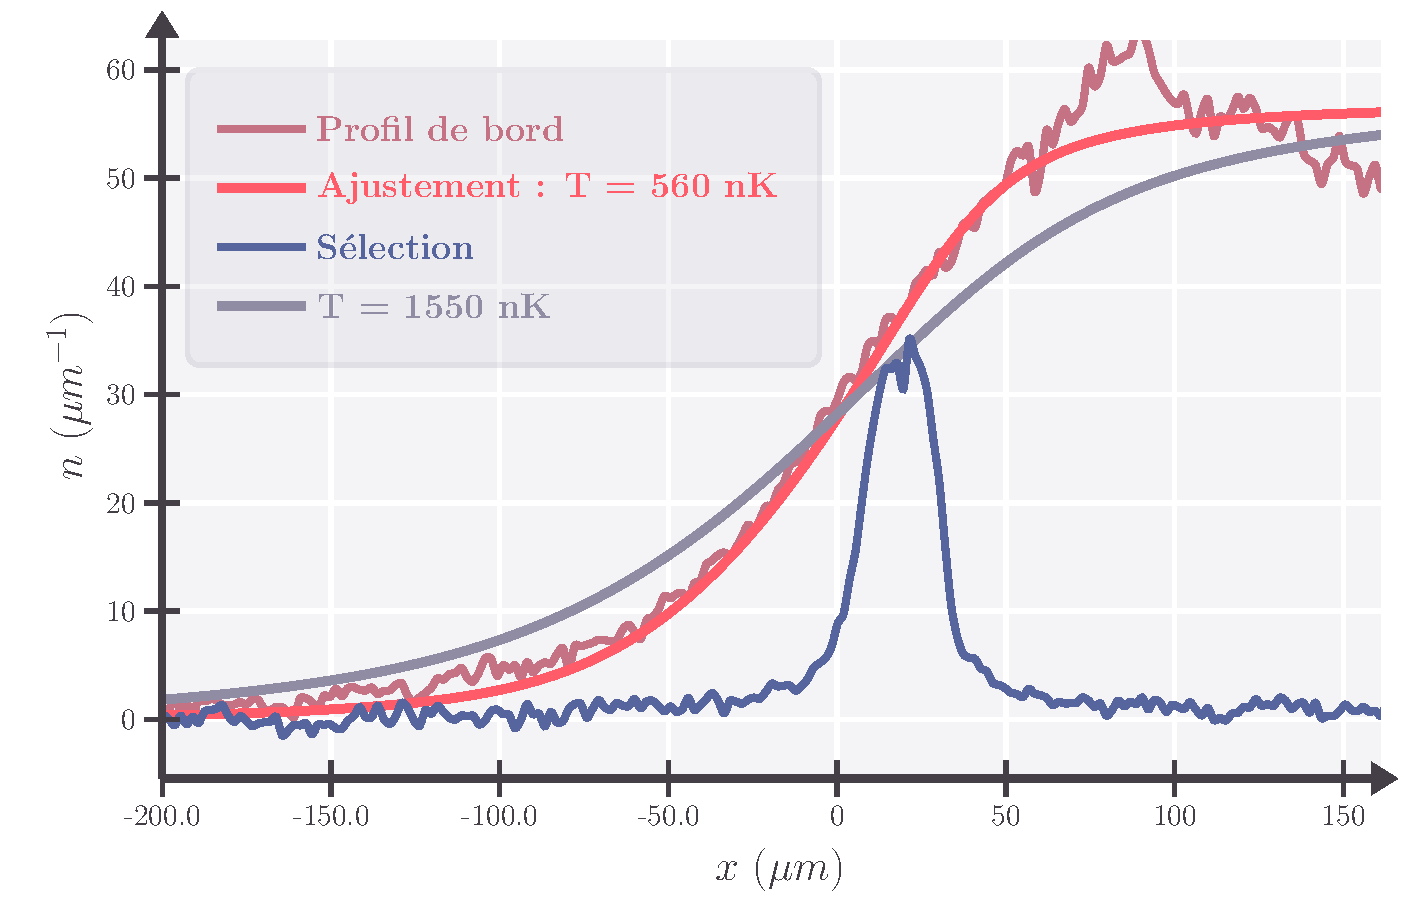
\includegraphics[width=0.5\textwidth , page = 1]{Figures}
    };
    \node[circle, draw=none, above=0cm of bord , shift={( -2.5cm , -0.5cm )} ] {(a)};
    
    \node[right=1mm of bord , shift={( -0.5cm , 0cm )}] (assy) {
        \includegraphics[width=0.5\textwidth , page = 2 ]{Figures}
    };
    \node[circle, draw=none, above=0cm of assy , shift={( -2.5cm , -0.5cm )}] {(b)};
\end{tikzpicture}
\caption{(a) {\it Profil de bord et tranche sélectionnée.} Le profil de bord après $18\,\mathrm{ms}$ est montré en rouge. L'ajustement thermique donne une température $T = 560\,\mathrm{nK}$ (orange). Le profil de densité mesuré $1\,\mathrm{ms}$ après la sélection de la tranche est en bleu. (b) {\it Asymétrie du profil d’expansion de la tranche.} Le profil de densité après une expansion pendant $\tau = 30\,\mathrm{ms}$ est comparé à son image miroir. Le centre de symétrie $x_s = -17\,\mu$m minimise la distance quadratique $\delta^2 = \int dx\, (\tilde{n}(x) - \tilde{n}(2x_s - x))^2$.}
\label{fig:simul_deformation}
\end{figure}

Pour aller au-delà de cette observation qualitative, nous effectuons un calcul GHD à l’échelle d’Euler du profil d’expansion, en supposant que l’état initial est thermique.  
La température est obtenue par ajustement du profil de bord avant la sélection de la tranche, comme indiqué en Fig.~\ref{fig:simul_deformation}(a), ce qui donne $T = 560$ nK.  
Le potentiel chimique est ajusté afin que la densité linéaire initiale corresponde à celle mesurée dans la région $x > 0$, avant l’élargissement du bord.  
À partir du profil initial, nous simulons à la fois l’élargissement du bord et l’expansion de la tranche en GHD, en supposant une découpe parfaite, c’est-à-dire $\nu(x,\theta) = 0$ pour $|x - x_0| > \ell/2$ et $\nu(x,\theta)$ inchangé sinon.  
La largeur $\ell$ est ajustée de sorte que le nombre d’atomes sélectionnés dans la simulation corresponde à celui mesuré expérimentalement après expansion, et on obtient $\ell = 24\,\mu$m.  

Le profil d’expansion simulé est montré en Fig.~\ref{fig:simul_expansion}(a).  
Il présente une forte asymétrie, comme attendu, avec un bord droit abrupt et une densité nulle au-delà d’un certain point.  
Cependant, cette chute est moins marquée que celle prédite pour la distribution locale des rapidités $\rho(x_0,\theta)$ à $x = x_0$. Deux effets contribuent à cet élargissement :  
(i) la distribution en rapidité n’est pas homogène à l’intérieur de la tranche, si bien que $\Pi(\theta)$ diffère de $\ell \rho(x_0,\theta)$, comme le montre la comparaison entre la ligne marron pleine et la ligne pointillée en Fig.~\ref{fig:simul_expansion}(a) ;  
(ii) le temps d’expansion est fini, de sorte que le profil observé $\tilde{n}(x, {\tau} )$ ne correspond pas exactement à $\Pi((x-x_0)/\tau)/\tau$, comme le montre la comparaison entre les courbes marron et rouge.



%l'ensemble $\{(x_g(1; \tau = 0^+) ,\ \theta(1; \tau = 0^+)) , \cdots , (x_g(q; \tau = 0^+) ,\ \theta(q; \tau = 0^+)) , (x_d(1; \tau = 0^+) ,\ \theta(1; \tau = 0^+)) , \cdots , (x_d(q; \tau = 0^+) ,\ \theta(q; \tau = 0^+)) \}$ ou $q$ est la taille des deux ensemble.



\begin{figure}[!htb]
\centering
\begin{tikzpicture}
    \node[rectangle, draw = none] (exp) at (0,0) {
       \includegraphics[width=0.5\textwidth , page = 3]{Figures}
    };
    \node[circle, draw=none, above=0cm of exp , shift={( -2.5cm , -0.5cm )} ] {(a)};
    
    \node[right=1mm of exp , shift={( -0.5cm , 0cm )}] (pi) {
       \includegraphics[width=0.5\textwidth , page = 4]{Figures}
    };
    \node[circle, draw=none, above=0cm of pi , shift={( -2.5cm , -0.5cm )}] {(b)};
\end{tikzpicture}
\caption{(a) {\it Profil de densité après expansion de la tranche : effets de la largeur finie et du temps d’expansion fini.} Courbe orange : profil obtenu par simulation GHD après expansion pendant $\tau = 30$ ms, avec $T = 560$ nK. Courbe marron : distribution asymptotique $\Pi((x - x_0)/\tau)/\tau$. Courbe pointillée noire : approximation $\ell \rho(x_0, (x - x_0)/\tau)/\tau$ dans le cas d’une tranche étroite. (b) {\it Comparaison aux données expérimentales.} En bleu : profil expérimental après expansion pendant $\tau = 30$ ms. En orange : simulation GHD avec $T = 560$ nK. En magenta : ajustement du profil expérimental donnant $T = 1550$ nK.}
\label{fig:simul_expansion}
\end{figure}

Nous comparons ensuite le profil d'expansion simulé par la GHD avec les données expérimentales. Comme montré en Fig.~\ref{fig:simul_expansion}(b), le profil prédit reproduit les principales caractéristiques du profil d'expansion observé expérimentalement. Des écarts atteignant 25\,\% sont cependant visibles dans la partie centrale du profil. Afin d'obtenir un meilleur accord entre données et calculs, nous avons ajusté le profil d'expansion expérimental avec le calcul GHD en utilisant la température de l'état initial comme paramètre d'ajustement. Le résultat, représenté par la ligne magenta dans la Fig.~\ref{fig:simul_expansion}(b), donne une température $T=1550$~nK, plus de deux fois supérieure à celle obtenue en ajustant le profil au bord. Le profil au bord calculé pour cette température n'est pas compatible avec le profil expérimental, comme le montre la Fig.~\ref{fig:simul_expansion}(b).

Une des raisons de l'échec de nos tentatives de reproduction du profil de densité après l'expansion de la tranche réside dans la présence de queues à droite du profil expérimental — voir le profil de densité dans la Fig.~\ref{fig:simul_expansion}(b). Ces queues sont absentes des calculs GHD à l’échelle d’Euler car la fonction d’occupation dans la tranche s’annule strictement au-delà d’une certaine rapidité. L’origine de ces queues reste incertaine. Elles pourraient être dues à des effets de bord associés à la procédure de sélection de tranche, les atomes en bordure étant chauffés par le faisceau de poussée. Il est également possible qu’un effet diffusif, non pris en compte dans la GHD à l’échelle d’Euler, intervienne au début de la déformation du bord, lorsque les gradients sont importants.

